% =====================================================================
%  Apresentacao curta - Despacho Hidrotermico e Manutencao de Geradores
%  Compilar:  latexmk -pdf apresentacao_curta.tex
%
%  Figuras: figuras/1_geracao_demanda.png   (visualizacao.py)
%           figuras/7_relax_and_cut.png     (plot_relax_and_cut.py, le lagrange_delayed_t504.npz)
%           figuras/6_manutencao.png        (plot_manutencao.py)
% =====================================================================
\documentclass[10pt,aspectratio=169]{beamer}

\usepackage[utf8]{inputenc}
\usepackage[T1]{fontenc}
\usepackage[brazilian]{babel}
\usepackage{amsmath,amssymb}
\usepackage{booktabs}
\usepackage{graphicx}
\usepackage{array}
\usepackage{ragged2e}

\usetheme{Boadilla}
\usecolortheme{seahorse}
\setbeamertemplate{navigation symbols}{}
\setbeamertemplate{caption}[numbered]
\setbeamerfont{block title}{size=\small}

% ---- Notacao (a mesma de apresentacao.tex) ----
\newcommand{\Gb}{\mathcal{G}}
\newcommand{\Hb}{\mathcal{H}}
\newcommand{\pH}{p^{H}}
\newcommand{\pT}{p^{T}}
\newcommand{\uH}{u^{H}}
\newcommand{\uT}{u^{T}}
\newcommand{\displaycompacto}{%
  \setlength{\abovedisplayskip}{2pt}%
  \setlength{\belowdisplayskip}{2pt}%
  \setlength{\abovedisplayshortskip}{2pt}%
  \setlength{\belowdisplayshortskip}{2pt}%
}

\title[Despacho e Manutenção]{Despacho Hidrotérmico e Manutenção de Geradores}
\subtitle{Relaxação Lagrangeana, \emph{Relax-and-Cut} e Programação por Restrições}
\author{Guilherme Bassous}
\institute{Otimização Combinatória II}
\date{novembro de 2026}

\begin{document}

\begin{frame}[plain]
  \titlepage
\end{frame}

% ===================== 1. PROBLEMA =====================
\begin{frame}{Despacho hidrotérmico: o problema}
  \begin{columns}[T]
    \begin{column}{0.47\textwidth}
      \footnotesize
      Programar a operação horária do sistema IEEE 14 barras, minimizando
      combustível, partidas e déficit, respeitando a rede e os reservatórios.

      \vspace{0.4em}
      \begin{block}{Sistema}
        \scriptsize
        \begin{itemize}\itemsep1pt
          \item 4 UHEs em cascata e 5 UTEs (42 a 450~R\$/MWh)
          \item 765~MW instalados; rede DC com 20 linhas
          \item Demanda aleatória com padrão de 24~h: média de 520~MW e pico de 715~MW
          \item Déficit a 3\,000~R\$/MWh
        \end{itemize}
      \end{block}

      \begin{block}{Instância: 3 semanas, $T = 504$}
        \centering\scriptsize
        \begin{tabular}{lr@{\qquad}lr}
          \toprule
          Contínuas & $36\,792$ & Restrições    & $51\,877$ \\
          Binárias  & $9\,576$  & \quad rampas  & $9\,054$  \\
          \emph{Total} & $46\,368$ & \quad tempo mínimo & $5\,019$ \\
          \bottomrule
        \end{tabular}
      \end{block}
    \end{column}
    \begin{column}{0.51\textwidth}
      \centering
      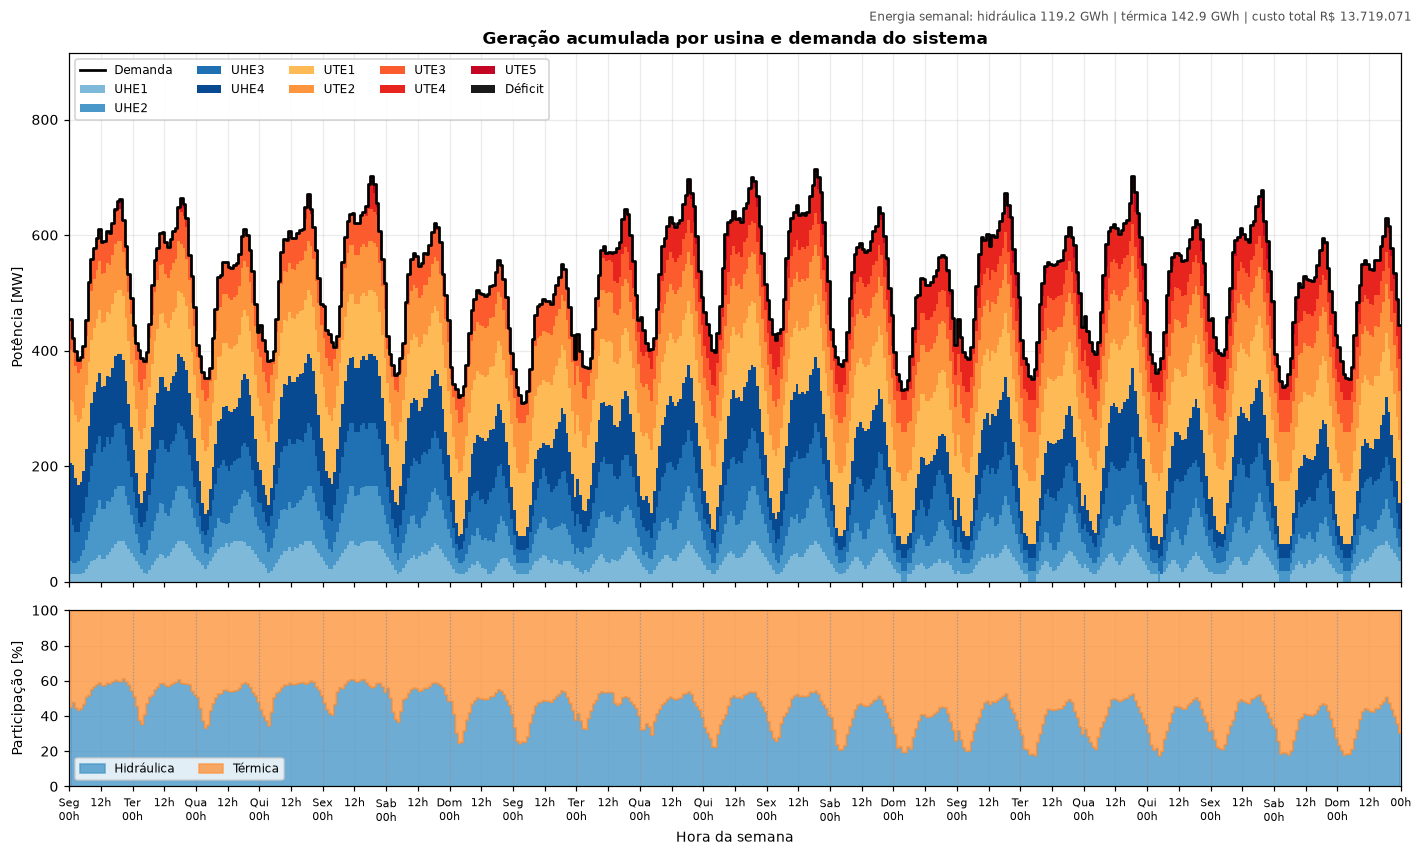
\includegraphics[width=\linewidth]{figuras/1_geracao_demanda.png}\\
      {\tiny Solução do MIP completo: geração por fonte \emph{vs.} demanda}
    \end{column}
  \end{columns}
\end{frame}

% ===================== 2. FORMULACAO =====================
\begin{frame}{Despacho hidrotérmico: formulação}
  \footnotesize
  \displaycompacto
  \begin{block}{Objetivo e rede}
    \[
      \min \sum_{g,t} \bigl( c_g \pT_{g,t} + c^{\text{par}}_g y_{g,t} \bigr)
           + c^{\text{def}} \sum_{n,t} r_{n,t}
      \quad\text{s.a.}\quad
      M^H \pH_t + M^T \pT_t + r_t - A f_t = D_t, \quad
      f_t = B A^\top \theta_t, \quad |f_{\ell,t}| \le \bar f_\ell
    \]
  \end{block}

  \begin{columns}[T]
    \begin{column}{0.49\textwidth}
      \begin{block}{Hidráulica}
        \begin{align*}
          & v_{u,t} = v_{u,t-1} + a_{u,t} - q_{u,t} - s_{u,t} + \textstyle\sum_{m} d_{m,t} \\
          & d_{u,t} = q_{u,t} + s_{u,t}, \qquad \pH_{u,t} = \rho_u q_{u,t} \\
          & \underline{p}^H_u \uH_{u,t} \le \pH_{u,t} \le \bar p^H_u \uH_{u,t} \\
          & |d_{u,t} - d_{u,t-1}| \le \Delta^H_u, \qquad v_{u,T} \ge \tfrac12 \bar v_u
        \end{align*}
      \end{block}
    \end{column}
    \begin{column}{0.49\textwidth}
      \begin{block}{Térmica}
        \begin{align*}
          & \underline{p}^T_g \uT_{g,t} \le \pT_{g,t} \le \bar p^T_g \uT_{g,t} \\
          & \uT_{g,t} - \uT_{g,t-1} = y_{g,t} - z_{g,t}, \quad y_{g,t} + z_{g,t} \le 1 \\
          & |\pT_{g,t} - \pT_{g,t-1}| \le R_g \\
          & \textstyle\sum_{s=t-t^{on}_g+1}^{t} y_{g,s} \le \uT_{g,t} \\
          & \textstyle\sum_{s=t-t^{off}_g+1}^{t} z_{g,s} \le 1 - \uT_{g,t}
        \end{align*}
      \end{block}
    \end{column}
  \end{columns}

  \vspace{0.2em}
  \scriptsize
  Binárias: $\uH$, $\uT$, $y$ (partida) e $z$ (desligamento).
\end{frame}

% ===================== 3. LAGRANGEANO =====================
\begin{frame}{Relaxação lagrangeana}
  \small
  \displaycompacto
  Dualizam-se \alert{rampas térmicas} ($5\,030$) e \alert{tempo mínimo} ($5\,019$),
  todas ``$\le$'', logo $\lambda \ge 0$:
  \[
    L(\lambda) = \min_{x \in X} \; c(x) + \lambda^\top (A x - b),
    \qquad
    z_{LD} = \max_{\lambda \ge 0} L(\lambda),
    \qquad
    z_{LP} \le z_{LD} \le z^*
  \]

  \vspace{0.2em}
  \begin{columns}[T]
    \begin{column}{0.45\textwidth}
      \begin{block}{Fica em $X$ (subproblema MIP)}
        \footnotesize
        Leis de Kirchhoff, balanço hídrico e cascata, \alert{rampa hidráulica},
        capacidade e geração mínima, lógica de transição.

        \vspace{0.3em}
        Os multiplicadores só alteram os custos lineares: o modelo é reaproveitado
        e apenas o objetivo é reescrito a cada iteração.
      \end{block}
    \end{column}
    \begin{column}{0.53\textwidth}
      \begin{block}{Método do subgradiente}
        \footnotesize
        $\lambda^0 = 0$; a cada iteração:
        \begin{enumerate}\itemsep1pt
          \item resolver o subproblema $\Rightarrow x^k$ e $L^k$
          \item $s^k = A x^k - b$
          \item $\alpha_k = \rho_k (UB - L^k) / \|s^k\|^2$ \hfill (Polyak)
          \item $\lambda^{k+1} = \max(0,\; \lambda^k + \alpha_k s^k)$
          \item $\rho_k \leftarrow \rho_k / 2$ após $p$ iterações sem melhora
        \end{enumerate}
      \end{block}
    \end{column}
  \end{columns}

  \vspace{0.2em}
  \footnotesize
  O subproblema é limitado por \emph{gap} ($10^{-3}$) e tempo ($60$~s).
\end{frame}

% ===================== 4. CORTES =====================
\begin{frame}{\emph{Relax-and-cut}: cortes de rampa}
  \footnotesize
  \displaycompacto
  \begin{block}{Família usada: rampa fortalecida pelo estado da máquina ($2G(T-1) = 5\,030$ cortes)}
    \[
      \pT_{g,t} - \pT_{g,t-1} \;\le\; R_g\, \uT_{g,t},
      \qquad\qquad
      \pT_{g,t-1} - \pT_{g,t} \;\le\; R_g\, \uT_{g,t-1}
    \]
    \scriptsize
    Válidos: com a máquina desligada a geração é zero e o lado esquerdo é $\le 0$;
    ligada, recai-se na rampa original. Dominam a rampa quando $\uT$ é fracionário.
  \end{block}

  \begin{columns}[T]
    \begin{column}{0.49\textwidth}
      \begin{block}{\emph{Delayed}}
        \scriptsize
        Subgradiente até convergir com o conjunto atual; separa em $x^k$ do melhor
        limite; dualiza até $200$ cortes por rodada; reinicia $\rho$ e o contador
        sem melhora ($5$ rodadas de $40$ iterações, no máximo).
      \end{block}
    \end{column}
    \begin{column}{0.49\textwidth}
      \begin{block}{\emph{Non-delayed}}
        \scriptsize
        Separa a cada iteração e dualiza na hora (até $50$ cortes). O contador zera
        quando entram cortes. Remove corte com $\lambda = 0$ e sem violação há $10$
        iterações.
      \end{block}
    \end{column}
  \end{columns}

  \vspace{0.3em}
  \begin{alertblock}{Limitação desta família}
    \scriptsize
    Em $x^k$ inteiro, um corte só é violado quando a própria rampa original é violada.
    A separação depende, então, de $x^k$ violar a rampa, e esse conjunto é pequeno.
    A família é polinomial; o uso típico de \emph{relax-and-cut} são famílias
    exponenciais, como as de rampa multiperíodo.
  \end{alertblock}
\end{frame}

% ===================== 5. RESULTADOS =====================
\begin{frame}{Lagrangeano e \emph{relax-and-cut}: resultados}
  \begin{columns}[T]
    \begin{column}{0.47\textwidth}
      \centering\scriptsize
      \setlength{\tabcolsep}{4pt}
      \begin{tabular}{lrrrr}
        \toprule
        Método & Limite (R\$) & Gap & It. & Cortes \\
        \midrule
        $z_{LP}$ & $13\,600\,868$ & $0{,}824\%$ & -- & -- \\
        Subgradiente & $13\,706\,559$ & $0{,}053\%$ & $40$ & -- \\
        \emph{Non-delayed} & $13\,706\,559$ & $0{,}053\%$ & $36$ & $9$ \\
        \emph{Delayed} & $13\,706\,781$ & $0{,}051\%$ & $80$ & $7$ \\
        \midrule
        Bound do MIP & $13\,712\,469$ & $0{,}010\%$ & -- & -- \\
        $UB$ do MIP & $13\,713\,838$ & -- & -- & -- \\
        \bottomrule
      \end{tabular}

      \vspace{0.5em}
      \raggedright
      \begin{block}{Leitura}
        \scriptsize
        \begin{itemize}\itemsep1pt
          \item $z_{LD} > z_{LP}$ implica que $X$ não tem a propriedade da integralidade.
          \item Os cortes não elevaram o limite: só $7$ a $9$ dos $5\,030$ foram separados.
          \item O \emph{gap} do subproblema (cerca de $13\,700$) supera o restante
                (cerca de $7\,000$), e o MIP completo dá limite melhor em $120$~s (as duas últimas linhas).
        \end{itemize}
      \end{block}
    \end{column}
    \begin{column}{0.51\textwidth}
      \centering
      \IfFileExists{figuras/7_relax_and_cut.png}{%
        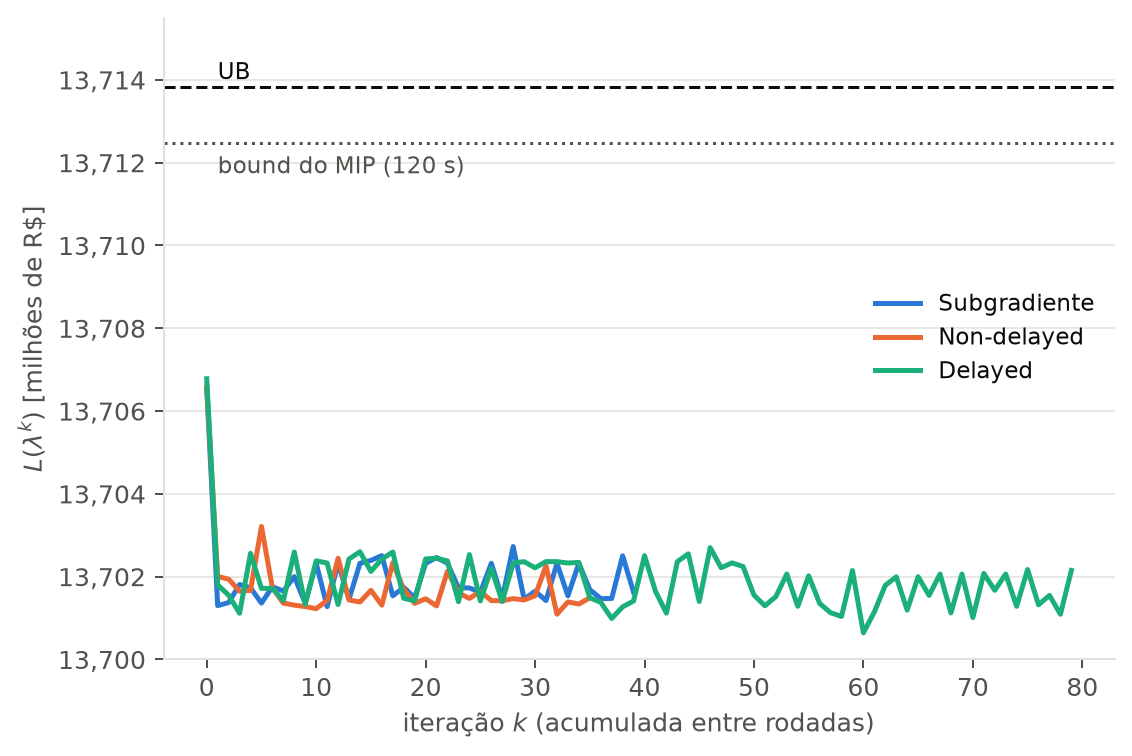
\includegraphics[width=\linewidth]{figuras/7_relax_and_cut.png}%
      }{\fbox{\parbox[c][3.2cm][c]{0.9\linewidth}{\centering\footnotesize\emph{figuras/7\_relax\_and\_cut.png}}}}
    \end{column}
  \end{columns}
\end{frame}

% ===================== 6. CP: PROBLEMA =====================
\begin{frame}{Manutenção de geradores: o problema}
  \small
  Escolher a semana de início da manutenção de cada unidade do sistema
  \alert{RTS-79} ao longo de $52$ semanas, sem comprometer a reserva, com
  equipes limitadas.

  \vspace{0.4em}
  \begin{columns}[T]
    \begin{column}{0.54\textwidth}
      \centering\scriptsize
      \begin{tabular}{lrrrr}
        \toprule
        Grupo & MW & Semanas & Equipes & Janela \\
        \midrule
        12 e 20 (9 un., óleo)  & 12--20 & 2 & 1 & 1--52 \\
        50 (6 un., hidro)      & 50     & 2 & 1 & 18--39 \\
        76 (4 un., carvão)     & 76     & 3 & 2 & 9--43 \\
        100 (3 un., óleo)      & 100    & 3 & 2 & 9--43 \\
        155 (4 un., carvão)    & 155    & 4 & 3 & 9--43 \\
        197 (3 un., óleo)      & 197    & 4 & 3 & 9--43 \\
        350 (1 un., carvão)    & 350    & 5 & 4 & 9--43 \\
        400 (2 un., nuclear)   & 400    & 6 & 5 & 9--30 \\
        \bottomrule
      \end{tabular}
    \end{column}
    \begin{column}{0.44\textwidth}
      \begin{block}{Restrições}
        \footnotesize
        \begin{itemize}\itemsep1pt
          \item Cada unidade para uma vez, sem interrupção, dentro da janela
          \item No máximo \alert{$7$ equipes} por semana
          \item Reserva de \alert{$15\%$}: capacidade disponível $\ge 1{,}15 \cdot$ pico da semana
          \item Na mesma barra, uma unidade por vez
        \end{itemize}
      \end{block}
    \end{column}
  \end{columns}

  \vspace{0.5em}
  \begin{block}{Objetivo e escala}
    \footnotesize
    Minimizar o \alert{pico de MW em manutenção}. São $32$ unidades e $3\,405$~MW
    instalados, com pico anual de $2\,850$~MW, $14\,086$~MW$\cdot$semana e
    $236$ equipes$\cdot$semana de manutenção.
  \end{block}
\end{frame}

% ===================== 7. CP: MODELO =====================
\begin{frame}{Manutenção de geradores: modelo CP}
  \small
  Um \alert{intervalo} por unidade: nenhuma variável indexada no tempo. O modelo usa
  CP Optimizer (\texttt{docplex.cp}).

  \vspace{0.5em}
  \centering\footnotesize
  \begin{tabular}{p{2.6cm}p{5.6cm}p{4.5cm}}
    \toprule
    Elemento & Expressão & \texttt{docplex} \\
    \midrule
    Manutenção de $i$ & $a_i$, duração $d_i$, dentro de $[e_i,\, l_i]$ & \texttt{interval\_var} \\
    Perfil de equipes & $E = \sum_i \text{pulse}(a_i,\, c_i)$ & \texttt{pulse} \\
    Perfil de MW & $W = \sum_i \text{pulse}(a_i,\, P_i)$ & \texttt{pulse} \\
    \midrule
    Limite de equipes & $0 \le E \le 7$ & \texttt{cumul\_range} \\
    Reserva na semana $t$ & $0 \le W \le \lfloor 3405 - 1{,}15 D_t \rfloor$ em $[t, t+1)$ & \texttt{always\_in} \\
    Mesma barra $b$ & $\text{noOverlap}(\{a_i : i \in b\})$ & \texttt{no\_overlap} \\
    \midrule
    Objetivo & $\min W^{\max}$, com $0 \le W \le W^{\max}$ & \texttt{cumul\_range}, \texttt{minimize} \\
    \bottomrule
  \end{tabular}

  \vspace{0.6em}
  \raggedright
  \begin{block}{Por que CP aqui}
    \footnotesize
    A função acumulada representa diretamente os recursos compartilhados no tempo, e
    \texttt{no\_overlap} propaga a exclusão sem \emph{big-M}. O limite de reserva varia
    a cada semana, o que \texttt{always\_in} expressa em uma restrição por semana.
    São $7$ barras com mais de uma unidade, cada uma com seu \texttt{no\_overlap}.
  \end{block}
\end{frame}

% ===================== 8. CP: RESULTADOS =====================
\begin{frame}{Manutenção de geradores: resultados}
  \centering
  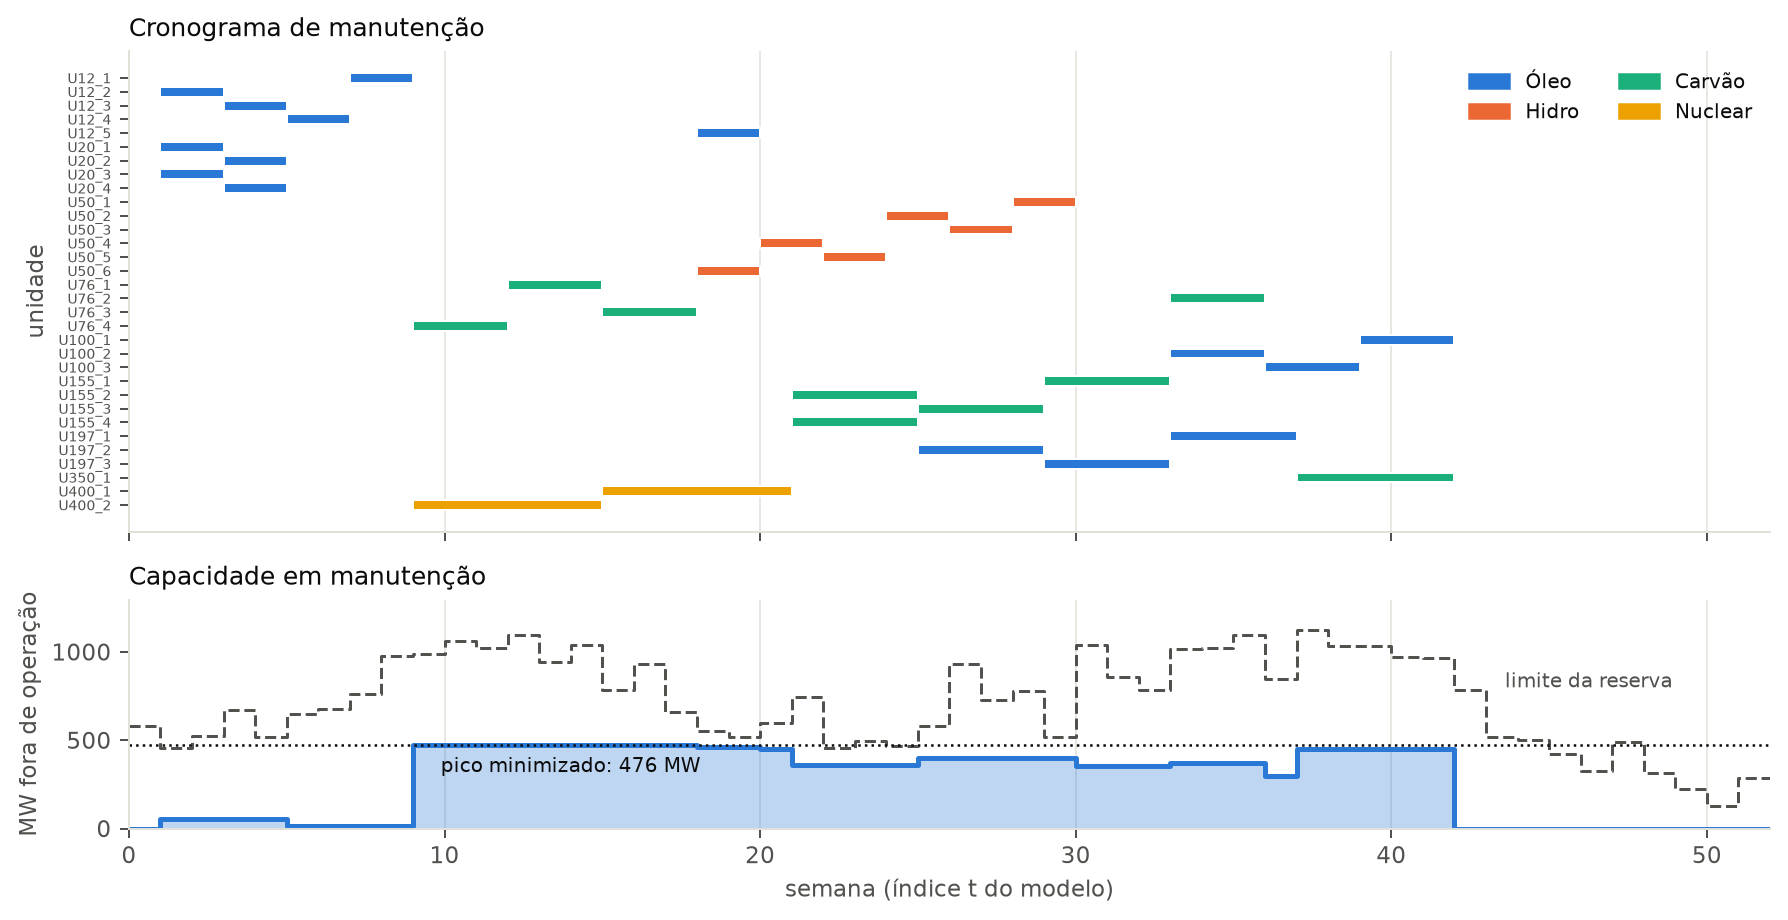
\includegraphics[height=0.62\textheight]{figuras/6_manutencao.png}

  \vspace{0.1em}
  \raggedright
  \begin{block}{Pico ótimo de \alert{476~MW}}
    \scriptsize
    \begin{itemize}\itemsep0pt
      \item Com $60$~s o solver encontra $476$~MW, com limite inferior de $400$ (\emph{gap} de $16\%$);
            com limite de $120$~s, prova a otimalidade de $476$.
      \item As $7$ equipes ficam saturadas em $23$ semanas. A menor folga da reserva é de $58$~MW.
    \end{itemize}
  \end{block}
\end{frame}

\end{document}
